Dear store manager, \newline

As we were studying the technological client groups, and creating mathematical models to describe the flash sale event, we came up with a solution that might help you hosting the event more conveniently.
We are here to provide you the new store layout that would reduce damage from the stampede of the customers during the flash sale. 
Our new floor plan use the technique of reducing the corner containing the products, which is where major damaged occur. Our plan tries to force the people to get into order by making the walkway straight and separating them into lots of groups independent to the others. 

\begin{center}
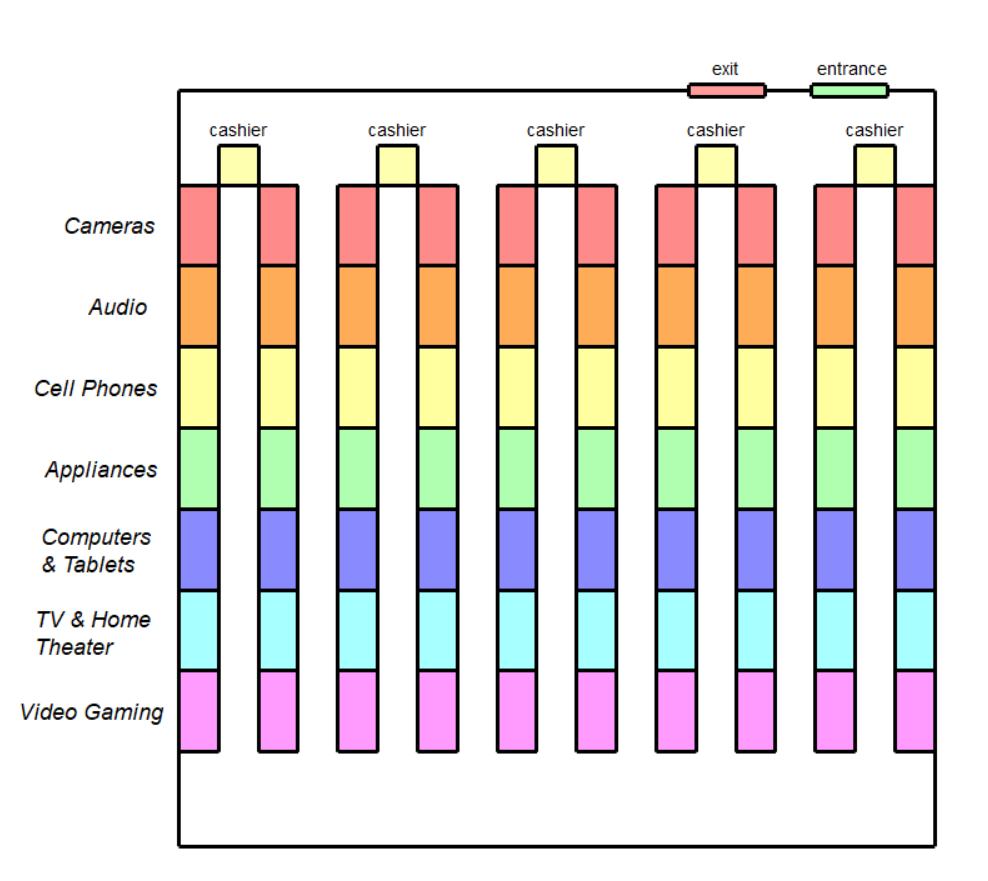
\includegraphics[width = 0.5\textwidth]{fig4.3.PNG}
\end{center}

From the picture, for each store block, the products will be placed only at the side adjacent to the walkway leading to the cashier. The other side would be just the wall leading customer to walk through the walkway to the bottom of the shopping hall.
Customers will enter at the entrance and walk into the space through the walkway between the wall, then make a u-turn into the space having the cashier at the end. They can pickup the products from here. 
The chaos inside the space containing the product would be less because the people are distributed into many groups and the walkway is straight.
The chaos at the entrance-exit area would be really bad but there's no products so there'll be no damage.
\newline

You can place the products according to the picture and the letter.
This would help minimize damage occured to your shop products and still give the same profit. 
\newline

Yours faithfully,\newline \par
Team 20200901.